\section{Preliminary Results}
\label{sec:preliminary_results}

A preliminary result would be about a rough estimation of a possible design of the fuel injector.

This implies to have a deep understanding of the chemical and physical properties of the alternative fuels and their combustion process.
Given that we don't have such a background in chemistry, nor we have the capability to perform a real CFD simulation, we can only try to replicate the results of the current state of the art just to have a starting point for our research.

\begin{figure}[H]
    \centering
    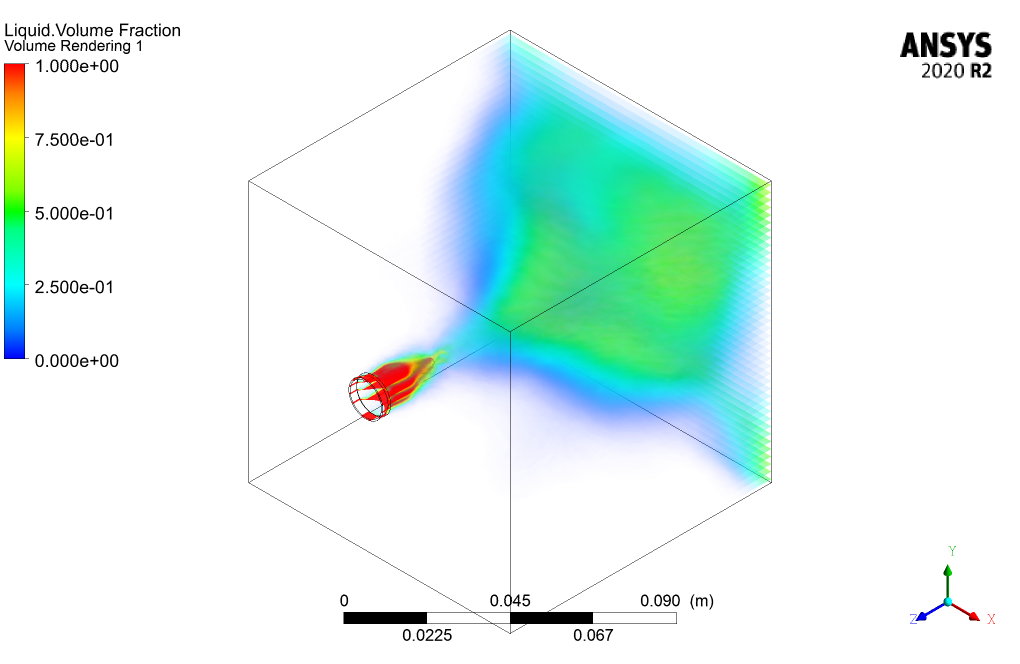
\includegraphics[width=0.8\textwidth]{img/injector_analysis_example.png}
    \caption{\href{https://www.mr-cfd.com/shop/fuel-injector-cfd-simulation-three-phase-flow/}{Analysis of a generic fuel injector.}}
    \label{fig:fuel_injector_analysis}
\end{figure}